\label{sec:model-usecase}
In this section we describe, with our model, the information disclosure and migration alteration attacks detailed in Section~\ref{sec:model-attacks}.
We prove the feasibility of detecting security violations with each attack, using the migration algorithms presented in Section~\ref{sec:model-migration}.
We describe a virtual topology and verify that the initial setup is respecting the security properties previously defined.
We do not include every single axiom used by SNARK for simplicity of reading.
% The full implementation of the use case in SNARK is described in Appendix~\ref{appendix:snark-code}.

We have implemented a simulator to generate the formal trace of the migration.
This work includes the topology, the algorithms used, the attacks on the migration process and the different rights users have on the infrastructure.

\subsection{Use case setup}
We have set up a network topology with six nodes, as depicted in Figure~\ref{fig:usecase-topo}

\begin{figure*}[htbp]



\tikzset{every picture/.style={line width=0.75pt}} %set default line width to 0.75pt        

\begin{tikzpicture}[x=0.75pt,y=0.75pt,yscale=-1,xscale=1]
%uncomment if require: \path (0,787.8333282470703); %set diagram left start at 0, and has height of 787.8333282470703

%Straight Lines [id:da7362912874212684] 
\draw [line width=1.5]    (217,249.33) -- (494,256) ;


%Straight Lines [id:da12239289508861262] 
\draw [line width=1.5]    (100,320) -- (217,249.33) ;


%Straight Lines [id:da40069379617810275] 
\draw [line width=1.5]    (226,398) -- (351,327) ;


%Straight Lines [id:da7000477419707168] 
\draw [line width=1.5]    (100,320) -- (226,398) ;


%Straight Lines [id:da4669112798901247] 
\draw [line width=1.5]    (230,405.33) -- (507,412) ;


%Straight Lines [id:da8512152422950844] 
\draw [line width=1.5]    (517,408) -- (510,260.33) ;


%Straight Lines [id:da12510362571528755] 
\draw [line width=1.5]    (514,413) -- (361,328.33) ;


%Straight Lines [id:da33197427034782157] 
\draw [line width=1.5]    (504,257) -- (369,328) ;


%Straight Lines [id:da19303419211846296] 
\draw [line width=1.5]    (363,321) -- (232,257) ;


%Image [id:dp07311130989675296] 
\draw (97.5,329) node  {
\includegraphics[width=52.5pt,height=52.5pt]{figures/router-158644_1280.png}};
%Image [id:dp12239452759411629] 
\draw (507.5,258.5) node  {
\includegraphics[width=52.5pt,height=52.5pt]{figures/router-158644_1280.png}};
%Image [id:dp678906579337467] 
\draw (218.5,413.75) node  {
\includegraphics[width=52.5pt,height=52.5pt]{figures/router-158644_1280.png}};
%Image [id:dp34355805397684036] 
\draw (507.5,413.75) node  {
\includegraphics[width=52.5pt,height=52.5pt]{figures/router-158644_1280.png}};
%Image [id:dp32408575207048074] 
\draw (360.5,329) node  {
\includegraphics[width=52.5pt,height=52.5pt]{figures/router-158644_1280.png}};
%Image [id:dp8786300863621592] 
\draw (218.5,258.5) node  {
\includegraphics[width=52.5pt,height=52.5pt]{figures/router-158644_1280.png}};


% Text Node
\draw (221,268) node  [align=left] {A};
% Text Node
\draw (102,338) node  [align=left] {B};
% Text Node
\draw (223,424) node  [align=left] {E};
% Text Node
\draw (364,340) node  [align=left] {C};
% Text Node
\draw (512,271) node  [align=left] {D};
% Text Node
\draw (514,424) node  [align=left] {F};


\end{tikzpicture}

\caption{Network topology of the use case.}
\label{fig:usecase-topo}

\end{figure*}


In addition to the topology, we name the time points of the different steps during the migration process based on the number of iterations (see Figure~\ref{fig:time-points}).
We define the first two basic time points time-0 and time-1 to respectively represent the initial situation and the beginning of the migration process. The last time point varies, depending on the length of execution of the migration.


\begin{figure}[htbp]
\centering
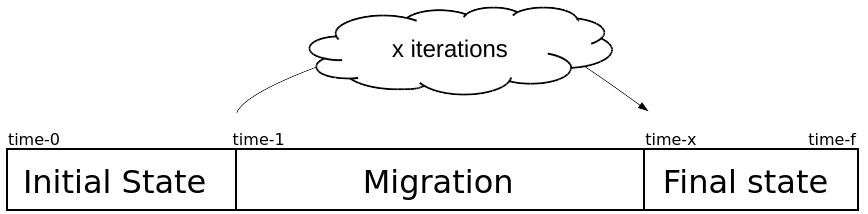
\includegraphics[scale=0.5]{figures/time-points-evolution} 
\caption{Time points of the migration process.\label{fig:time-points}}
\end{figure}

\subsection{Initial Situation}
In this section, we consider the network topology prior to any migration.
We solely have the axioms related to the virtual network, the corresponding users, and the data carried across the network.
We formulate our question to SNARK and verify that the confidentiality is already established prior to the migration (question and answer in Listing~\ref{lst:init-conf-q} and~\ref{lst:init-conf-a}, respectively).



\begin{lstlisting}[caption=SNARK question to validate the initial situation., label=lst:init-conf-q,captionpos=b] 
(find-all '(ans ?d.data ?t.time-interval)
 '(and
 (data-confidentiality ?d.data ?t.time-interval)
(non-empty ?t.time-interval))
 :name 'data-confidentiality-preservation-conjecture
 :num-answers 1
 :time-limit 30  
 :print-derived :print)


(find-all '(ans ?d.data ?t.time-interval)
 '(and
 (config-integrity ?d.data ?n.node ?t.time-interval)
(non-empty ?t.time-interval))
 :name 'config-integrity-preservation-conjecture
 :num-answers 1
 :time-limit 30  
 :print-derived :print)
\end{lstlisting}

%\GB{could you comment a bit about what piece of SNARK response  in Lst.~\ref{lst:init-conf-a} gives away the result?}
The interpretation of results provided by SNARK depends on how the question has been formulated.
Listing~\ref{lst:init-conf-q} contains requests for the format of the answer.
For the data confidentiality, line 1 describes what are the variables we are looking for. Lines 2-4 describes what SNARK has to prove, \ie the data confidentiality property that holds on a non empty time interval.
Lines 5-8 are options passed to SNARK for the resolution.
We have a similar request in lines 11-18 for the configuration integrity property.

We execute SNARK to find the proofs of these two questions.
Lines 5 and 11 of Listing~\ref{lst:init-conf-a} hold the answers.
We can establish from line 5 that data-1 has its confidentiality respected (and it is the only one used in our experiment).
At line 11, we have proven that conf-1 is not compromised either (and it is the only one used as well).
% The same goes for all the other nodes of the topology, for the sake of brevity, these proofs have been omitted.
%but we do not provide the print out in this paper.

\begin{lstlisting}[caption=SNARK validating the initial situation, label=lst:init-conf-a,captionpos=b] 
(Row 69
(OR ($$TIME-PP-NOT-BEFORE TIME-0 TIME-4) 
(= (SOME-USER1 DATA-1 (MAKE-INTERVAL TIME-0 TIME-4)) USER-2))
(RESOLVE 66 NON-EMPTY-IF-TIME-POINTS-ORDERED)
Answer (ANS (ANS DATA-1 (MAKE-INTERVAL TIME-0 TIME-4)))) 


(Row 480
   (AFTER TIME-2 TIME-3)
   (REWRITE (RESOLVE 235 0-IS-BEFORE-1) :CODE-FOR-$$TIME-PP-COMPOSITION)
   Answer (ANS (ANS CONF-1 (MAKE-INTERVAL TIME-0 TIME-1)))) 
\end{lstlisting}


\subsection{Information Disclosure attack}
%\GB{are both attacks directed against both migration algorithms}
%\FC{No, but I forgot to mention that we assign an attack per algorithm}
This attack considers two users, one legitimate and one attacker.
The attacker is a collocated user.
In this scenario, the iterative migration algorithm is used.
During the initial phase, only the legitimate user is active.
The migration process starts and nodes and links are being migrated, one after another.
At some point during the migration, the attacker will start his attack to gain access to the data carried through the VN.
This results into the generation of two predicates, one about the attacker reading the data, and the other about him not being authorized to do so. 
When the migration process ends, the data has been compromised.
In SNARK, the piece of data has been named data-1 and the migration ends at time point time-9.
We formulate our question to SNARK at line 1 from Listing~\ref{lst:not-data-conf-q}, specifying which terms we are looking for.
Similarly to previous examples, lines 3-4 represent the violation of the confidentiality over a non-empty time interval.

% \begin{figure}[h]
% \centering
% \includegraphics[scale=0.5]{not-data-confidentiality-question}
% \caption{SNARK question to detect the data confidentiality violation.\label{fig:not-data-conf-q}}
% \end{figure}
% \begin{figure}[h]
% \centering
% \includegraphics[scale=0.5]{not-data-confidentiality-answer}
% \caption{SNARK detecting the data confidentiality violation\label{fig:not-data-conf-a}}
% \end{figure}
\begin{lstlisting}[caption=SNARK question to detect the data confidentiality violation., label=lst:not-data-conf-q,captionpos=b] 
   (find-all '(ans ?d.data ?t.time-interval)
             '(and
       (not(data-confidentiality ?d.data ?t.time-interval))
         (non-empty ?t.time-interval))
         :name 'data-conf-preservation-conjecture
         :num-answers 1
         :time-limit 30
         :print-derived :print)
;;; search for a data-confidentiality breach:
;;; find all data for which data-confidentiality has been maintained

\end{lstlisting}

We can see that SNARK confirms the data confidentiality violation at line 12 from Listing~\ref{lst:not-data-conf-a}.
Since the attack started during the migration (i.e after time point time-1), SNARK detects the beginning of the confidentiality violation at time point time-4.
Line 10 highlights that the attacker does not have the authorization to read the data.
%\GB{could you point out directly which line you are referring to by labeling and referring to independent lines in the listing?}

\begin{lstlisting}[caption=SNARK detecting the data confidentiality violation., label=lst:not-data-conf-a,captionpos=b] 
(Row 2112  
(OR
 (NOT
  (= (MAKE-INTERVAL TIME-0 ?X.TIME-POINT)
   (MAKE-INTERVAL (MAX-TIME ?Y.TIME-POINT ?Z.TIME-POINT) (MIN-TIME ?U.TIME-POINT ?V.TIME-POINT))))
 (NOT (SETLINK0 NODE-B ?W.NODE (MAKE-INTERVAL ?Y.TIME-POINT ?U.TIME-POINT)))
 (NOT (SETLINK ?W.NODE NODE-A (MAKE-INTERVAL ?Z.TIME-POINT ?V.TIME-POINT)))
 ($$TIME-PP-NOT-BEFORE TIME-9 (MIN-TIME TIME-1 ?X.TIME-POINT)) ($$TIME-PP-NOT-BEFORE TIME-4 TIME-9)
 (NOT (= (MAKE-INTERVAL TIME-4 TIME-9) (MAKE-INTERVAL TIME-0 TIME-9))) ($$TIME-PP-NOT-BEFORE TIME-4 TIME-9)
 (DATA-ISAUTHORIZED ATTACKER DATA-1 (MAKE-INTERVAL TIME-4 TIME-9)))
   (RESOLVE 1938 18)
   Answer (ANS (ANS DATA-1 (MAKE-INTERVAL TIME-4 TIME-9)))) 
\end{lstlisting}


\subsection{Migration alteration attack}
Exploiting the physical nodes leverages other aspects of the security of the infrastructure.
The initial situation is similar to the previous scenario but we use the move-based migration algorithm instead.
The attacker is located in the network infrastructure and can render physical nodes unavailable to trigger the migration process. He will then intercept and modify the configuration sent by the hypervisor. 
Therefore, the $conf\_integrity$ property is not respected anymore.

We implement in SNARK the $conf\_integrity$ property, as depicted in Listing~\ref{lst:conf-integrity-definition}.\\
Lines 1-3 define the equivalence between the $conf\_integrity$ property and the other predicates.
Line 4 defines a logical AND between the following predicates:
Line 5 defines \textit{?t.t-int}, a time interval as the intersection of all the time intervals expressed in the following predicates.
Line 11 assigns controller \textit{?c.controller} to node \textit{?n.node}.
Line 14 defines \textit{?p.path} as the path between \textit{?c.controller} and \textit{?n.node}.
Line 17 assigns configuration \textit{?d.data} to node \textit{?n.node}.
Line 20 represents preservation of the integrity of configuration data \textit{?d.data}.
Note that we modeled the implication ($\Rightarrow$) defined in Section~\ref{sec:security_prop} as a logical conjunction.
Line 23 ensures that \textit{?t.t-int} is not empty.

\begin{lstlisting}[caption=SNARK definition of the configuration integrity., label=lst:conf-integrity-definition,captionpos=b] 
(implied-by
  (config-integrity 
     ?d.data ?n.node ?t.t-int)
  (and
    (= ?t.t-int
       (intersection
    	  (time-i ?r1.t-pt ?r2.t-pt)
    	  (time-i ?s1.t-pt ?s2.t-pt)
    	  (time-i ?u1.t-pt ?u2.t-pt)
    	  (time-i ?v1.t-pt ?v2.t-pt)))
    (is-hypervisor-of
       ?c.controller ?n.node 
       (time-i ?r1.t-pt ?r2.t-pt))
    (is-path 
	   ?c.controller ?p.path ?n.node
       (time-i ?s1.t-pt ?s2.t-pt))
    (conf-of-node
	   ?d.data ?n.node
       (time-i ?u1.t-pt ?u2.t-pt))
    (d-integrity
	   ?d.data
       (time-i ?u1.t-pt ?u2.t-pt))
    (non-empty ?t.t-int)))

\end{lstlisting}

We formulate in Listing~\ref{lst:not-conf-int-q} the question for SNARK.
Line 1 represents the format of the answer, here we look for which configuration is being compromised. In lines 2-4 we search for the violation of the $conf\_integrity$ property over a non empty interval. Similarly to other questions, lines 5-8 represent parameters for SNARK to use in the resolution.

\begin{lstlisting}[caption=SNARK question to detect the configuration integrity violation., label=lst:not-conf-int-q,captionpos=b] 
   (find-all '(ans ?d.data ?t.time-interval)
             '(and
       (not(conf-integrity ?d.data ?n.node ?t.time-interval))
               (non-empty ?t.time-interval))
             :name 'conf-integrity-violation-conjecture
             :num-answers 1
             :time-limit 5
                     :print-derived :print)
\end{lstlisting}

The configuration integrity breach is then proven by SNARK in Listing~\ref{lst:not-conf-int-a} for conf-1 at line 8 between time points time-3 and time-4 .
Similarly to the previous information disclosure scenario, the attack starts after the beginning of the migration process, as shown by the answer term starting at time-3.

The proofs related to the other security properties are identical in essence, thus we do not include them here.
% SNARK finds the beginning of the attack on node-a starting at time point time-3.
%\GB{again, please provide line numbers for the reviewer to ``see something''}

\begin{lstlisting}[caption=SNARK detecting the configuration integrity violation., label=lst:not-conf-int-a,captionpos=b] 
(Row 197
   FALSE
   (REWRITE (RESOLVE 154 2-IS-BEFORE-3) :CODE-FOR-$$TIME-PP-INTERSECTION)
   Answer 
(ANSWER-IF (= (CONF-1 (MAKE-INTERVAL TIME-1 TIME-4) (MAKE-INTERVAL TIME-1 TIME-3)) PROCESS-1)
 (ANS (ANS (MAKE-INTERVAL TIME-3 TIME-4))) (ANS (ANS (MAKE-INTERVAL TIME-2 TIME-3)))))
)
((ANS (ANS CONF1 (MAKE-INTERVAL TIME-3 TIME-4)))

\end{lstlisting}

